\documentclass{beamer}
\usetheme{metropolis}

\usepackage[dvipdfmx]{}

\title{チームで \TeX を書く方法}
\author{佐藤 礼於}
\date{June 29, 2018}

\begin{document}
\frame{\maketitle}

\section{\TeX \ with Git}

\begin{frame}{そもそも \TeX とは}
  組版のためのソフトウェア.
  このままだと書くのが面倒なので,マイクロパッケージを組み込んだ \LaTeX が広く使われている.
\end{frame}

\begin{frame}{何故 \TeX なのか}
  一番の利点は,\alert{全てがコードであること}.

  つまりGitで管理できる.
  また後述する文章校正の自動化ができる.

  プロジェクト学習の報告書に於いては,WGがテンプレートを用意しているので,それに合わせて文章を入れれば良い.
  いちいちスタイルについて頭を悩ますことなく,文章作成に集中できる.
\end{frame}

\begin{frame}{\TeX のファイル分割}
  \textbackslash usepackage\{subfiles\}

  \textbackslash subfile\{sections/aaa\}

  という感じで分割できる.

  これによりGitを使った共同執筆が容易になる.

  なお,1つのファイルは同時に1人しか触らない方が無難.
\end{frame}


\section{応用}

\begin{frame}{CIとは}
  Continuous Integrationの略.
  プログラムのテストを継続的に行う仕組み.

  \begin{itemize}
    \item Circle CI
    \item Travis CI
    \item Jenkins
  \end{itemize}
\end{frame}

\begin{frame}{Circle CI}
  
\includegraphics[width=4cm, bb=0 0 140 137]{img/circle-logo-stacked-black.png}

  \begin{itemize}
    \item ロゴがカッコイイ
    \item デフォでAmazon S3を用意してくれてる
  \end{itemize}

  ⇒ \alert{ビルドしたPDFを置いておける}
\end{frame}

\begin{frame}{\TeX とCI}
  CIの基本的な機能,任意のスクリプトを実行し,その結果をテストの結果とする.

  つまり,\alert{CIに \TeX のビルドをさせて,上手くビルドできたかできなかったかを知れれば良い}.

  \begin{itemize}
    \item ついでにビルドしたPDFをSlackに送ってもらう
    \item ついでにLintしてもらう
  \end{itemize}
\end{frame}

\begin{frame}{Lintとは}
  プログラムの書き方を矯正するための仕組み.

  \begin{itemize}
    \item スペース or タブ
    \item タブ幅はどうするか
    \item \{は改行するか
  \end{itemize}
\end{frame}

\begin{frame}{TextLint}
  文章のチェックに特化したLintツール.

  \begin{itemize}
    \item 日本語の文法チェック
    \item 表記揺れ,IT系専門用語のチェック
  \end{itemize}
\end{frame}

\begin{frame}{GitHubとCircle CI}
  簡単に連携できる.

  テストが通らなければ,プルリクのマージを阻止できる
  →masterのコードは常にビルドできる状態に保てる.

  また,Lintの結果をプルリクのConversation/Checksに投稿できる.
\end{frame}

\begin{frame}{図にするとこうなる}
  % https://drive.google.com/file/d/1Wm2u-g6rbPoUxQg2zA11x--jE5Wfsh-m
  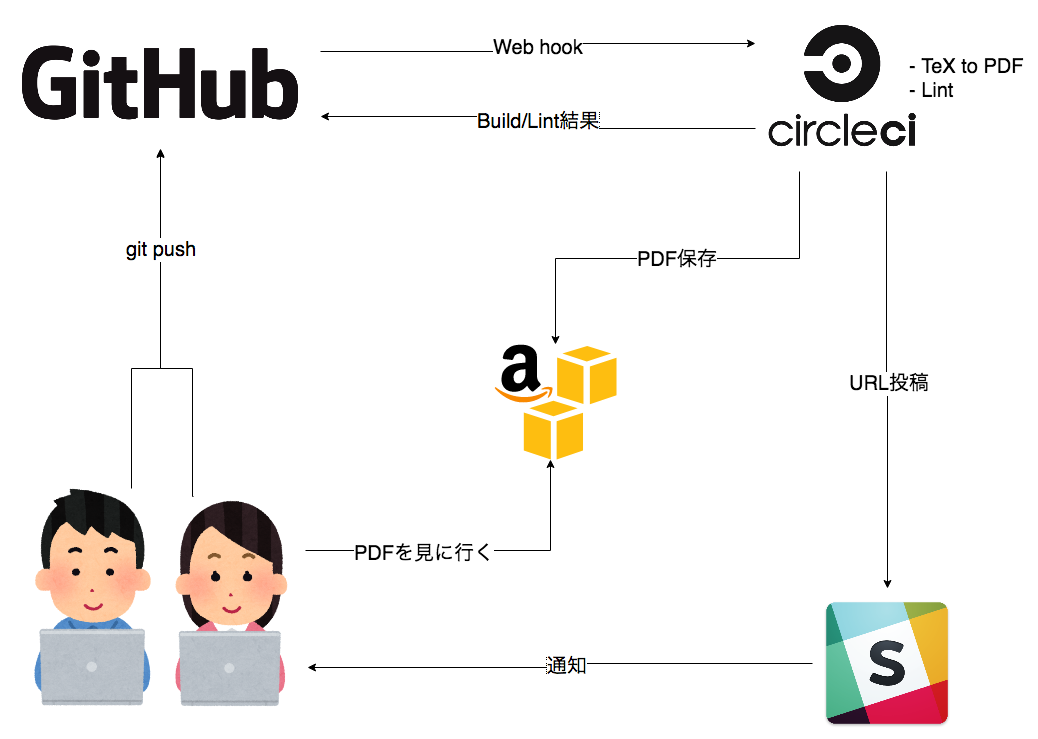
\includegraphics[width=\textwidth, bb=0 0 1038 739]{img/ideal_sequence.png}
\end{frame}

\frame{\centering \Large \alert{皆で楽しく} \TeX を書こう}

\end{document}
